\documentclass[]{report}

\voffset=-1.5cm
\oddsidemargin=0.0cm
\textwidth = 480pt

\usepackage{framed}
\usepackage{subfiles}
\usepackage{enumerate}
\usepackage{graphics}
\usepackage{newlfont}
\usepackage{eurosym}
\usepackage{amsmath,amsthm,amsfonts}
\usepackage{amsmath}
\usepackage{color}
\usepackage{amssymb}
\usepackage{multicol}
\usepackage[dvipsnames]{xcolor}
\usepackage{graphicx}
\begin{document}


HibColl Videos

%% --------------------%% --------------------%% --------------------%% --------------------%% ------------------------

1.A  Converting from Decimal to Binary
1.B  Converting from Decimal to Hexadecimal
1.C  Converting from Binary to Decimal
1.D  Converting from Hexadecimal to Decimal
1.E  Binary Addition
1.F  Binary Subtraction

%% --------------------%% --------------------%% --------------------%% --------------------%% ------------------------

2.A  Membership Tables
2.B  Venn Diagrams
2.C  Set differences and symmetric difference
2.D  
2.E



\chapter{Number Systems}
\subsection{Significant Digits}
There are three rules on determining how many significant figures are in a number: Non-zero digits are always significant. Any zeros between two significant digits are significant. A final zero or trailing zeros in the decimal portion ONLY are significant.

\section{Floating Point Notation}



In computing, floating point describes a method of 
representing an approximation of a real number in a 
way that can support a wide range of values. 


The numbers are, in general, represented approximately 
to a fixed number of significant digits (the mantissa) and scaled using an exponent. 

In essence, computers are integer machines and are capable of representing real numbers only by using complex codes. The most popular code for representing real numbers is called the IEEE Floating-Point Standard .
The term floating point is derived from the fact that there is no fixed number of digits before and after the decimal point; that is, the decimal point can float. There are also representations in 
which the number of digits before and after the decimal point is set, called fixed-point representations. In general, floating-point representations are slower and less accurate than fixed-point representations, but they can handle a larger range of numbers.







\end{enumerate}


% \item The Fibonacci sequence $f_n$ is defined recursively by the rule
%   \begin{equation*}
%     \begin{cases}
%       f_0&=0\\
%       f_1&=1\\
%       f_n&=a_{n-1}+a_{n-2}
%     \end{cases}
%   \end{equation*}

%   \begin{enumerate}
%   \item
%     Write a program to evaluate the Fibonacci sequence and hence evaluate $f_{50}$.
%   \item
%     Let the sequence $g_n$ be defined as the ratio
%     \begin{equation*}
%       g_n = \frac{f_{n+1}}{f_n}
%     \end{equation*}
%     Write a program to evaluate the first $50$ terms of the sequence $g_n$.
%   \item
%     Assumming that the sequence $g_n$ has a limit $\phi$, find this limit.
%   \end{enumerate}


\subsection*{Floating Point Notation}
(Demonstration on white board)


\section*{Part A: Number Systems - Binary Numbers}
\begin{enumerate}
\item Express the following decimal numbers as binary numbers.
\begin{multicols}{4}
\begin{itemize}
\item[i)] $(73)_{10}$
\item[ii)] $(15)_{10}$
\item[iii)] $(22)_{10}$
\end{itemize}
\end{multicols}

All three answers are among the following options.
\begin{multicols}{4}
\begin{itemize}
\item[a)] $(10110)_{2}$ %22
\item[b)] $(1111)_{2}$ %15
\item[c)] $(1001001)_{2}$ %73
\item[d)] $(1000010)_{2}$ %64
\end{itemize}
\end{multicols}

\item Express the following binary numbers as decimal numbers.
\begin{multicols}{4}
\begin{itemize}
\item[a)] $(101010)_{2}$
\item[b)] $(10101)_{2}$
\item[c)] $(111010)_{2}$
\item[d)] $(11010)_{2}$
\end{itemize}
\end{multicols}
\item Express the following binary numbers as decimal numbers.
\begin{multicols}{4}
\begin{itemize}
\item[a)] $(110.10101)_{2}$
\item[b)] $(101.0111)_{2}$
\item[c)] $(111.01)_{2}$
\item[d)] $(110.1101)_{2}$
\end{itemize}
\end{multicols}
\item Express the following decimal numbers as binary numbers.
\begin{multicols}{4}
\begin{itemize}
\item[a)] $(27.4375)_{10}$  %
\item[b)] $(5.625)_{10}$
\item[c)] $(13.125)_{10}$
\item[d)] $(11.1875)_{10}$
\end{itemize}
\end{multicols}
\end{enumerate}

\section*{Part B: Number Systems - Binary Arithmetic}
%http://www.csgnetwork.com/binaddsubcalc.html
(See section 1.1.3 of the text)
\begin{enumerate}
\item Perform the following binary additions.
\begin{multicols}{2}
\begin{itemize}
\item[a)] $(110101)_{2}$ + $(1010111)_{2}$
\item[b)] $(1010101)_{2}$ + $(101010)_{2}$
\item[c)] $(11001010)_{2}$ + $(10110101)_{2}$
\item[d)] $(1011001)_{2}$ + $(111010)_{2}$
\end{itemize}
\end{multicols}

\item Perform the following binary subtractions.
\begin{multicols}{2}
\begin{itemize}
\item[a)] $(110101)_{2}$ - $(1010111)_{2}$
\item[b)] $(1010101)_{2}$ - $(101010)_{2}$
\item[c)] $(11001010)_{2}$ - $(10110101)_{2}$
\item[d)] $(1011001)_{2}$ - $(111010)_{2}$
\end{itemize}
\end{multicols}


\item Perform the following binary multiplications.
\begin{multicols}{2}
\begin{itemize}
\item[a)] $(1001)_{2}\times( 1000)_{2}$  % 9 by 8
\item[b)] $(101)_{2}\times(1101)_{2}$ % 5 by 11
\item[c)] $(111)_{2}\times(1111)_{2}$ % 7 by 15
\item[d)] $(10000)_{2}\times(11001)_{2}$    %16 by 25
\end{itemize}
\end{multicols}

\newpage

\item Perform the following binary multiplications.
%\begin{multicols}{2}
%\begin{itemize}
%\item[a)] $(1001000)_{2} \div ( 1000)_{2}$
%\item[b)] $(101101)_{2} \div (1001)_{2}$
%\item[c)] $(1001011000)_{2} \div (101000)_{2}$
%\item[d)] $(1100000)_{2} \div (10000)_{2}$
%\end{itemize}
%\end{multicols}

\begin{enumerate}
\item Which of the following binary numbers is the result of this binary division: $(10)_{2} \times ( 1101)_{2}$. % % (2) /  (13)
\begin{multicols}{2}
\begin{itemize}
\item[a)] $(11010)_{2}$ %26
\item[b)] $(11100)_{2}$ %28
\item[c)] $(10101)_{2}$ %21
\item[d)] $(11011)_2$ %27
\end{itemize}
\end{multicols}
\item Which of the following binary numbers is the result of this binary division: $(101010)_{2} \times( 111 )_{2}$. % (4) /  (6)
\begin{multicols}{2}
\begin{itemize}
\item[a)] $(11000)_{2}$ %24
\item[b)] $(11001)_{2}$ %25
\item[c)] $(10101)_{2}$ %21
\item[d)] $(11011)_2$ %27
\end{itemize}
\end{multicols}
\item Which of the following binary numbers is the result of this binary division: $(1001110)_{2}\times ( 1101 )_{2}$. % (9) /  (3)
\begin{multicols}{2}
\begin{itemize}
\item[a)] $(11000)_{2}$ %24
\item[b)] $(11001)_{2}$ %25
\item[c)] $(10101)_{2}$ %21
\item[d)] $(11011)_2$ %27
\end{itemize}
\end{multicols}
\end{enumerate}

%----------------------------------------------------------------%

\item Perform the following binary divisions.
%\begin{multicols}{2}
%\begin{itemize}
%\item[a)] $(1001000)_{2} \div ( 1000)_{2}$
%\item[b)] $(101101)_{2} \div (1001)_{2}$
%\item[c)] $(1001011000)_{2} \div (101000)_{2}$
%\item[d)] $(1100000)_{2} \div (10000)_{2}$
%\end{itemize}
%\end{multicols}

\begin{enumerate}
\item Which of the following binary numbers is the result of this binary division: $(111001)_{2} \div ( 10011)_{2}$. % (57) /  (19)
\begin{multicols}{2}
\begin{itemize}
\item[a)] $(10)_2$ %2
\item[b)] $(11)_{2}$ %3
\item[c)] $(100)_{2}$ %4
\item[d)] $(101)_{2}$ %5
\end{itemize}
\end{multicols}
\item Which of the following binary numbers is the result of this binary division: $(101010)_{2} \div ( 111 )_{2}$. % (42) /  (7)
\begin{multicols}{2}
\begin{itemize}
\item[a)] $(11)_2$ %3
\item[b)] $(100)_{2}$ %4
\item[c)] $(101)_{2}$ %5
\item[d)] $(110)_{2}$ %6
\end{itemize}
\end{multicols}
\item Which of the following binary numbers is the result of this binary division: $(1001110)_{2} \div ( 1101 )_{2}$. % (78) /  (13)
\begin{multicols}{2}
\begin{itemize}

\item[a)] $(100)_{2}$ %4
\item[b)] $(110)_{2}$ %6
\item[c)] $(111)_{2}$ %7
\item[d)] $(1001)_2$ %9
\end{itemize}
\end{multicols}
\end{enumerate}


\end{enumerate}








% \newpage
\section*{Part D: Natural, Rational and Real Numbers}
\begin{itemize}
\item $\mathbb{N}$ : natural numbers (or positive integers) $\{1,2,3,\ldots\}$
\item $\mathbb{Z}$ : integers $\{-3,-2,-1,0,1,2,3,\ldots\}$
\begin{itemize}
\item (The letter $\mathbb{Z}$ comes from the word \emph{Zahlen} which means ``numbers" in German.)
\end{itemize}
\item $\mathbb{Q}$ : rational numbers
\item $\mathbb{R}$ : real numbers
\item $\mathbb{N} \subseteq \mathbb{Z } \subseteq \mathbb{Q} \subseteq \mathbb{R}$
\begin{itemize}
\item (All natural numbers are integers. All integers are rational numbers. All rational numbers are real numbers.)
\end{itemize}
\end{itemize}




\subsection{Irrational Numbers}
An irrational number cannot be expressed as a ratio between two numbers and it cannot be written as a simple fraction because there is not a finite number of numbers when written as a decimal. Instead, the numbers in the decimal would go on forever, without repeating.



In mathematics, the cardinality of a set is a measure of the "number of elements of the set". For example, the set A = {2, 4, 6} contains 3 elements, and therefore A has a cardinality of 3.







\section{Set Theory}
\begin{enumerate}
\item The Universal Set $\mathcal{U}$
\item Union
\item Intersection
\item Set Difference
\item Relative Difference
\end{enumerate}



DE Muorgan's Laws (Useful for Propositions)

membership tables

proof by truth tables
AND
OR
NOT
Set difference
symmetric difference



\newpage


Harmonic Mean

\[ H_x = \frac{ n }{ \frac{ 1 }{ x_1 } + \frac{ 1 }{ x_2 } + \cdots + \frac{ 1 }{ x_n } } \]

2,4,6,8
> 1/mean(1/a)
[1] 3.84
> 1/a
[1] 0.5000000 0.2500000 0.1666667 0.1250000
> sum(1/a)
[1] 1.041667
> sum(1/a)*24
[1] 25
> 96/25
[1] 3.84



\subsection{Functions}
Consider the floor function $f : R \rightarrow Z$ given the rule

\[ f(x) = \lfloor \frac{x+1}{2} \rfloor \]

\begin{enumerate}
\item evaluate $f(6)$ and $f(-6)$
\item Show that f(x) is not one-to-one
\item 
\end{enumerate}

%----------------------------------------%

\subsection{Functions}
Evaluate $f(6)$ 


\[ f(x) = \lfloor \frac{x+1}{2} \rfloor \]


\[ f(6) = \lfloor \frac{\boldsymbol{6}+1}{2}\rfloor = \lfloor  \frac{7}{2}\rfloor\]


\[  \lfloor 3.5 \rfloor  = 3  \]


%----------------------------------------%

\subsection{Functions}
Evaluate $f(-6)$ 


\[ f(x) = \lfloor \frac{x+1}{2} \rfloor \]


\[ f(6) = \lfloor \frac{\boldsymbol{-6}+1}{2}\rfloor = \lfloor  \frac{-5}{2}\rfloor\]


\[  \lfloor -2.5 \rfloor  = -3  \]






% http://www.textbooksonline.tn.nic.in/books/12/std12-bm-em-1.pdf


\subsection{Discrete Maths : Relations}

\begin{itemize}
\item A relation $R$ from a set A to a set B is a subset of the
\textbf{cartesian product} A x B. 
\item Thus R is a set of \textbf{ordered pairs} where
the first element comes from A and the second element comes
from B i.e. $(a, b)$
\end{itemize}

%-----------------------------------%

\subsection{Discrete Maths : Relations}

\begin{itemize}

\item  If $(a, b) \in R$ we say that $a$ is related to $b$ and write $aRb$.
\item If $(a, b) \notin R$, we say that $a$ is not related to $b$ and write $aRb$. CHECK
\item If
$R$ is a relation from a set $A$ to itself then we say that ``$R$ is a relation
on $A$".
\end{itemize}

%-----------------------------------%

\subsection{Discrete Maths : Relations}

%% %% - \vspace{-2cm}
\textbf{Example}
\begin{itemize}
\item Let $A = \{2, 3, 4, 6\}$ and $B = \{4, 6, 9\}$
\item Let R be the relation from A to B defined by \textit{\textbf{xRy}} if $x$
divides $y$ exactly.
\end{itemize}


%-----------------------------------%

\subsection{Discrete Maths : Relations}

%% %% - \vspace{-0.7cm}
\textbf{Example}
\begin{itemize}

\item Let $A = \{2, 3, 4, 6\}$ and $B = \{4, 6, 9\}$
\item Let R be the relation from A to B defined by \textit{\textbf{xRy}} if $x$
divides $y$ exactly.
\item  Then
\[R = {(2, 4), (2, 6), (3, 6), (3, 9), (4, 4), (6, 6)}\]
\end{itemize}



%------------------------------------------------------------------------%
\section{Arrow Diagrams}

\begin{itemize}

\item Domain
\item Co-Domain
\item Range
\end{itemize}
\[  f(x) : \mbox{Domain} \rightarrow \mbox{Co-Domain} \]
\[  f(x) : \mathbb{R} \rightarrow \mathbb{R} \]
%----------------------------------------------------------- %
\newpage
\subsection*{Polynomial Functions (4.1.5)}

\begin{itemize}
\item[Constants] $(P_0)$
\item[Linear Functions] $(P_1)$
\item[Quadratic Functions] $(P_2)$
\item[Cubic Functions] $(P_3)$
\end{itemize}


\subsection*{Equality of Functions (4.1.6)}
\[f(x) = g(x) \]




%------------------------------------------------------%
\subsection{Exercise} 
$h(x): \mathbb{R} \rightarrow \mathbb{R}$ 
$g(x): \mathbb{R} \rightarrow \mathbb{R}$

\[f(x) = sqrt(x)\]
\[g(x) = \sqrt{3}{x+2}\]
\[h(x) = 2^x\]

\begin{itemize}
\item Is the function $h(x)$ an \textit{onto} function?
\item determine the inverse function of $h(x)$ and $g(x)$
\item Simplify the following function.
\[ j(x) = \mbox{log}_4(h(6x))\]
\end{itemize}
%--------------------------------------------%
\subsection{Onto Functions}
Definition: If every element in the co-domain of the function has an ancestor, the function is said to be "onto".
An onto function has the property that the domain is equal to the co-domain.


\textbf{Example 4.26 Page 53}

%------------------------------------------------------------------------%
\section{\textit{One-to-One} Functions and \textit{Onto} Functions}

\subsection{Invertible Functions}
\begin{itemize}
\item One-to-One Function
\item Onto Function
\end{itemize}

Onto Functions : Range and Co-Domain are equivalent

\subsection{Inverting a Function}

\begin{itemize}
\item[$\bullet$] You are given $f(x)$ in terms of $x$
\item[$\bullet$] Re-arrange the equation so that $x$ is given in terms of $f(x)$
\item[$\bullet$] Replace $x$ with $f^{-1}(x)$ and $f(x)$ with $x$
\end{itemize}

\subsubsection{Example}
\begin{itemize}
\item[$\bullet$]Determine the inverse function of $f(x)$. Re-arrange the equation so that $x$ is given in terms of $f(x)$
\[  f(x): \mathbb{R} \rightarrow \mathbb{R}  \mbox{   } f(x)  = \sqrt{x+1} \]
\item[$\bullet$] Square both sides of the equation.
\[[f(x)]^2 = x+1 \]
\item[$\bullet$] Subtract 1 from both sides of the equation. We have the equation written in terms of x.
\[f(x)^2-1 = x \]
\item[$\bullet$] Replace $x$ with $f^{-1}(x)$ and $f(x)$ with $x$
\[x^2-1 = f^{-1}(x) \]
\item[$\bullet$] 
Re-arrange equation and specify domain and co-domain.
\[ f(x): \mathbb{R} \rightarrow \mathbb{R}  \mbox{   }  f^{-1}(x) = x^2-1  \]
\end{itemize}
% \[ f(x)  = \sqrt{x+1} \]
% \[f(x)^2 = x+1 \]
% \[f(x)^2-1 = x \]
% \[x^2-1 = f^{-1}(x) \]
\newpage
\section{Big O-Notation}

%------------------------------------------------------------------------%
% Section 4 Functions
% http://doc.gold.ac.uk/~maa01km/solutions/tut4sol.pdf
\begin{itemize}
\item[(b)] Let $S$ be the set of all 4 bit binary strings. 

The function $f : S \rightarrow \mathbb{Z}$
is defined by the rule:
\[f(x) = \mbox{the number of zeros in x}\]
for each binary string $x \in S$.\\
Find:
\begin{enumerate}
\item the number of elements in the domain
\item $f(1000)$
\item the set of pre-images of 1
\item the range of $f$.
\end{enumerate}
\item[(c)]
\end{itemize}
\newpage
\begin{itemize}
\item[4.a] $ \lfloor x - y \rfloor = \lfloor x \rfloor - \lfloor y \rfloor$
\item[4.b]
\item[4.c]
\end{itemize}
\newpage
%------------------------------------------------------------------------%
\section{Section 4 Functions}

\subsection{Invertible Functions}
A function is invertible if it fulfils two criteria
\begin{itemize}
\item The function is \textbf{\textit{onto}},
\item The function is \textbf{\textit{one-to-one}}.
\end{itemize}

State the conditions to be satisfied by a function
$f : X \leftarrow Y$ for it to have an inverse function
$f^{-1} : Y \leftarrow X$.
%---------------------------------------------------------%

$\lceil \frac{x^2+1}{4} \rceil$
where $f : A \rightarrow \textbf{Z}$
\begin{itemize}
\item[(i)] Find $f(4)$ and the ancestors of 3.
\item[(ii)] Find the range of $f$.
\item[(iii)] Is f invertible? Justify your answer
\end{itemize}

Given $f : \textbf{R} \rightarrow \textbf{R}$ where f(x) =3x-1,define fully
the inverse of the function f ,i.e.$f^{-1}$. 
State the value of $f^{-1}(2)$



\section{Laws of Exponents}
Here are the Laws (explanations follow):

LawExample
x1 = x61 = 6
x0 = 170 = 1
x-1 = 1/x4-1 = 1/4
xmxn = xm+nx2x3 = x2+3 = x5
xm/xn = xm-nx6/x2 = x6-2 = x4
(xm)n = xmn(x2)3 = x2×3 = x6
(xy)n = xnyn(xy)3 = x3y3
(x/y)n = xn/yn(x/y)2 = x2 / y2
x-n = 1/xnx-3 = 1/x3
%--------------------------------------------------%
Z Score
\[ Z = \frac{X - \mu}{\sigma} \]
%--------------------------------------------------%




%-------------------------------------------------------%


%% --------------------
\subsection{Exercises}

Showing your workings, use the rules of indices and logarithms to give the following two expression in their simplest form.
\bigskip
\begin{itemize}
\item \textbf{Exercise 1}
\[ 4 \cdot 2^x - 2^{x+1} \]
\item \textbf{Exercise 2}
\[  \frac{\mbox{ln}(2) + \mbox{ln}(2^2) + \mbox{ln}(2^3)  + \mbox{ln}(2^4) + \mbox{ln}(2^5)  }  {\mbox{ln}(4)}  \]
\end{itemize}
%% --------------------

%-------------------------------------------------------%
%% --------------------
\subsection{Exercise 1}

\[ 4 \cdot 2^x - 2^{x+1} \]

\textbf{Remarks:}\\
\textit{(looking at the second term)}
\begin{itemize}
\item[1] Using the following rule
\[ a^b \cdot a^c = a^{(b+c)}  \] 
\item[2] Using this rule in reverse we can say
\[ 2^{x+1} = 2^x \cdot 2^1  = 2\cdot (2^x) \] 
\end{itemize}
\[ 4 \cdot 2^x - 2^{x+1} \mbox{   } = \mbox{   } (4 \cdot 2^x) -  (2\cdot 2^{x}) \]
%% --------------------

%-------------------------------------------------------%
%% --------------------
\subsection{Exercise 1}

%% %% - \vspace{-0.9cm}

\textbf{Remarks:}
\begin{itemize}
\item[3] This expression is in the form 
\[ (a  \cdot b ) - ( c  \cdot b) \]
which can be re-expressed as follows 
\[ (a - c\sqrt{b} )  \cdot b \]
\end{itemize}
\[ (4 \cdot 2^x) -  (2\cdot 2^{x}) = (4-2)  \cdot 2^{x} \]
\[   = 2 \cdot 2^x = 2^{x+1}\]
%% --------------------
%-------------------------------------------------------%

%% --------------------
\subsection{Exercise 2}


\[  \frac{\mbox{ln}(2) + \mbox{ln}(2^2) + \mbox{ln}(2^3)  + \mbox{ln}(2^4) + \mbox{ln}(2^5)  }  {\mbox{ln}(4)}  \]
Useful Rule of Logarithms
\[  \mbox{ln}(a^b)  = b\cdot \mbox{ln}(a)  \]
\[  \frac{\mbox{ln}(2) + 2 \cdot \mbox{ln}(2) + 3 \cdot\mbox{ln}(2)  + 4 \cdot \mbox{ln}(2) + 5 \cdot \mbox{ln}(2)  }  {\mbox{ln}(4)}  \]
%% --------------------
%--------------------------------------%
%% --------------------
\subsection{Exercise 2}

Adding up all the terms in the numerator

\[  \frac{1\cdot\mbox{ln}(2) + 2 \cdot \mbox{ln}(2) + 3 \cdot\mbox{ln}(2)  + 4 \cdot \mbox{ln}(2) + 5 \cdot \mbox{ln}(2)  }  {\mbox{ln}(4)} \]  \[= \frac{15 \cdot \mbox{ln}(2) }{\mbox{ln}(4)} \]


%% --------------------

%--------------------------------------%
%% --------------------
\subsection{Exercise 2}

Our expression has now simplified to 
\[\frac{15 \cdot \mbox{ln}(2) }{\mbox{ln}(4)} \]

We can simplify the denominator too

\[ \mbox{ln}(4) =  \mbox{ln}(2^2) = 2 \cdot \mbox{ln}(2) \]


%% --------------------

%--------------------------------------%
%% --------------------
\subsection{Exercise 2}

Our expression has now simplified to 
\[\frac{15 \cdot \mbox{ln}(2) }{\mbox{ln}(4)} = \frac{15 \cdot \mbox{ln}(2) }{2 \cdot \mbox{ln}(2)} \]

We can divide above and below by $\mbox{ln}(2)$ to get our final answer


\[ \frac{15 \cdot \mbox{ln}(2) }{2 \cdot \mbox{ln}(2)} = \frac{15}{2} = 7.5 \]

%% --------------------

%% --------------------
%-----------------------------------------------------%
\section*{Prepositional Logic}


%-------------------------------------------------------------------------%
\newpage
\section{Section 3 Logic}
\subsection{Logical Operations}
\begin{itemize}
\item $\neg p$ the negation of proposition $p$.
\item $p \wedge q$ Both propositions p and q are simultaneously true (Logical State AND)
\item $p \vee q $ One of the propositions is true, or both (Logical State : OR)
\item $p \otimes q$ Only one of the propositions is true (Logical State : exclusive OR (i.e XOR)
\end{itemize}
\begin{center}
\begin{tabular}{|c|c|c|c|c|}
\hline
p & q & $p \vee q$ & $q \wedge p$ & $p \otimes q$ \\
\hline
0 & 0 & 0 & 0 & 0 \\
0 & 1 & 1 & 0 & 1\\
1 & 0 & 1 & 0 & 1 \\
1 & 1 & 1 & 1 & 0\\
\hline
\end{tabular}
\end{center}
%---------------------------------------------------------%
\section{Conditional Connectives}
Construct the truth table for the proposition $p \rightarrow q$.

\begin{center}
\begin{tabular}{|c|c|c|c|}
\hline
p & q & $p \rightarrow q$ & $q \rightarrow p$ \\
\hline
0 & 0 & 1& 1 \\
0 & 1 & 1 & 0 \\
1 & 0 & 0 & 1 \\
1 & 1 & 1 & 1 \\
\hline
\end{tabular}
\end{center}

% Question 1 - numbers - Started
% Question 2 - Sets - Not Started
% Question 3 - Logic - Not Started
% Question 4 - Functions - Started
% Question 5 - Graphs
% Question 6 - Digraphs and Relations
% Question 7 - 
% Question 8 -
% Question 9
% Question 10 - Matrices - STARTED

\subsection*{Question 4}
%2001 Question 4
\begin{center}
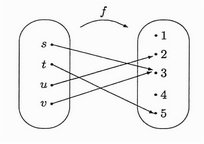
\includegraphics[scale=0.55]{HibCollArrow.jpg}
\end{center}




\subsection*{Question 10}

(a) Given the following adjacency matrices A and B where
%A =
%
%1 0 1
%0 1 2
%1 2 0
%
% ,B =
%
%1 2 0
%2 0 1
%0 1 1

%MAKE NO

%--------------------------------------------%

(i) Say whether or not the graphs they represent are isomorphic.
(ii) Calculate A2 and A4 and say what information each gives about the graph
corresponding to A. [6]
(b) (i) Write down the augmented matrix for the following system of equations.

\[2x + y - z = 2\]
\[x - y + z = 4\]
\[x + 2y + 2z = 10\]
(ii) Use Gaussian elimination to solve the system. [4]



\subsection*{Dice Rolls}
Consider rolls of a die. What is the universal set?

\[ \mathcal{U} = \{1,2,3,4,5,6\} \]

%--------------------------------------%

\subsection*{symbols}
$\varnothing$,
$\forall$,
$\in$,
$\notin$,
$\cup$

\chapter{Sequences and Series, and Proof by Induction}
\section{Sequence and Series and Proof by Induction}


\[\sum (n^2) \]



%----------------------------------------------------%
\subsection*{Binary and Hex}
\begin{itemize}
\item[1A.1] Coverting from Binomial to Decimal
\item[1A.2] Converting to Decimal
\item[1A.3] Priority of Operation
\item[1A.4] 
\end{itemize}

\subsection*{Numbers}
\begin{itemize}
\item[1B.1] Real Numbers
\item[1B.2] Rational Numbers
\item[1B.3] Floating Point Aritmetic
\item[1B.4] 
\end{itemize}
%================================================================ %



%------------------------------------------------------------------------- %
\section{Revision Questions}



\[  2^ 4 = 2 \times 2 \times 2 \times 2 = 16 \]

\[  5^ 3 = 5 \times 5 \times 5 =125 \]

\subsubsection{Special Cases}

Anything to the power of zero is always 1

\[  X^ 0 = 1 \mbox{ for all values of X} \]

Sometimes the power is a negative number.

\[  X^{-Y} = { 1 \over X^Y}  \]

Example 
\[  2^{-3} = { 1 \over 2^3} = { 1 \over 8}  \]


%====================================== %
\newpage
\begin{center}
\huge{Mathematics for Computing}\\
{ Session 2 : Set Theory}
\end{center}



%====================================== %
\newpage
\begin{center}
\huge{Mathematics for Computing}\\
{ Session 3 : Logic}
\end{center}
% %\subfile{session03a.tex}
% % \subfile{session03d.tex}
% % \subfile{DM0305DeMorgans.tex}

%============================================ 

% % \subfile{session06a.tex}
% % \subfile{session06e-antisymmetricrelations.tex}
% % \subfile{session06f.tex}


%----------------------------------------- %
\section{Video 6}

%\frametitle{Inequality Symbols}

Convert the following statements into symbols:

\begin{itemize}
\item $\sqrt{2}$ is less than 1.5 and greater than 1.4
\item $\sqrt{2}$ is greater than or equal to 5
\end{itemize}



%------------------------------------------------------------------------- %
% Floating Point Notation

\chapter{Session 4}
\section*{Invertible Functions}

Necessary Condtions for Invertibility of a Function
\begin{itemize}
\item The function must be one-to-one
\item The fucntion must be onto.
\end{itemize}

%-------------------------- %
%-------------------------- %
%Section 5 Graph Theory

\section*{Equivalence Relations}

%%%%%%%%%%%%%%%%%%%%%%%%%%%%%%%%%%%%%%%%%%%%%%%%%%%%%%%%%%%%%%%%5

\subsection*{Session 04:Functions}
\begin{itemize}
\item Definitions
\end{itemize}

\begin{itemize}
\item[Domain]
\item[Co-domain]
\item[Image]
\item[Ancestor]
\item[Range]
\end{itemize}

\subsection*{Part A : Functions}
Given a real number $x$, say how the floor of x  $\lfloor x \rfloor$ is defined.
\begin{itemize}
\item[(i)] Find the values of $\lfloor 2.97 \rfloor$ and $\lfloor -2.97 \rfloor$.
\item[(ii)] Find an example of a real number $x$ such that $\lfloor 2x \rfloor  \neq 2\lfloor x \rfloor$, justifying your answer.
\end{itemize}



\subsection*{Absolute Value Function (4.1.3)}


\begin{itemize}
\item The absolute value of some real number $x$ is denoted $|x|$.
\item If the number is positive, the asbolute value is the same number.
\item If the number is negative, the asbolute value is the number without the minus sign.
\item $|2|=2$
\item $|-2| = 2$
\end{itemize}
\subsection*{Floor and Ceiling Function (4.1.4)}
\subsection*{Polynomial Functions (4.1.5)}

\begin{itemize}
\item[Constants] $(P_0)$
\item[Linear Functions] $(P_1)$
\item[Quadratic Functions] $(P_2)$
\item[Cubic Functions] $(P_3)$
\end{itemize}


\subsection*{Equality of Functions (4.1.6)}
\[f(x) = g(x) \]



\subsection*{One-to-One Functions (4.2.3)}
$f(x)$, must be \emph{One-to-One} and \emph{Onto}



\subsection*{Exponential and Logarithmic Functions (4.3)}

The Laws of Logarithms
\begin{itemize}
\item
\item $log_b(x^y) = y \times log_b(x)$
\item
\item
\end{itemize}
%================================================================== %

\subsection*{Big O-notation}
Comparing the size of Functions (4.4)
%----------------------------------------- %
%----------------------------------------- %


Using O-notations

\subsection*{Power Notation (4.4.2)}




% %------------------------------------------------------


\section{Section 4 Functions}


%---------------------------------------------------------%



\section*{Functions}
\begin{itemize}
\item Domain of a Function
\item Range of a function
\item Inverse of a function
\end{itemize}
\begin{itemize}
\item one-one (surjective)
\item onto (bijective)
\end{itemize}
%------------------------------------------------%






\section{Video 7 : Numbers}


\begin{description}
\item[mantissa]
\item[abscissa]
\item[radix point]
\end{description}

\begin{itemize}
\item Number Systems
\item Set Theory
\item Function
\item 
\item Graph Theory
\end{itemize}



\begin{itemize}
\item Digraphs
\item Set Theory
\item Function
\item Probability
\item MAtrices
\end{itemize}



%\frametitle{(1.4.1) Decimal to Binary Conversion}
\begin{itemize}
\item Continuously divide the decimal number by 2.
\item Keep record of the remainder, either 0 or 1.
\item The sequence of remainders is the binary number required.
\end{itemize}

%------------------------------------------%

%\frametitle{Hexadecimal Numbers}
\begin{itemize}
\item Hex Characters $\{0,1,2,3,4,5,6,7,8,9,A,B,C,D,E,F\}$
\item 
\end{itemize}

%-------------------------------------%

%\frametitle{Relatiional Operators}
\begin{itemize}
\item $\neq$ Not Equal
\item < Less than
\item > greater than
\item $\geq$ greater than or equal to
\item $\leq$ Not Equal to
\end{itemize}

%------------------------------------------%

%\frametitle{Frame Name}
\begin{itemize}
\item Natural Numbers $\{1,2,3,4, \ldots\}$
\item Integers $\{\ldots,-2,-1,0,1,2,3,\ldots\}$
\item Rational Numbers e.g $4/7$ , $11/25$
\item Real Numbers Any number e.g. $3.1415$
\end{itemize}



%----------------------------------------------%

\begin{itemize}
\item Decmal Number Systesm
\begin{itemize}
\item Base 10
\end{itemize}

\item Binary Number Systems
\begin{itemize}
\item Base 2
\item allowable characters are {0.1} only
\end{itemize}
\item Base 16 Hexadecimal
\begin{itemize}
\item Use all of the decimal digits, in addition to 6 more A,B~,D,D,E,F
\end{itemize}
(where might you see this  - specifying colours RGB Numbers
\end{itemize}

%============================================================= %
For example FF in hexadecimal is is 255 in decimal 


Rational Numbers

Natural Numbers indies
Integers Z


%--------------------------------------------%

Computing a binary number

Useful
{
\begin{center}
\begin{tabular}{|c|c|}
\hline $2^0 = 1 $ & $2^4 = 16  $ \\ 
\hline $2^1 = 2 $ & $2^5 = 32$ \\ 
\hline $2^2 = 4 $ & $2^6 = 64$ \\ 
\hline $2^3 = 8 $ & $ 2^7 = 128$ \\ 
\hline 
\end{tabular} 
\end{center}
}


%============================================================= %
\newpage




Firslly determine the highest power

Suppose the number we wish to convert is 58

Hwhat is the highest power of two that deivides



\end{document}
